\documentclass[10pt,a4paper]{article}

\usepackage[utf8]{inputenc}
\usepackage[T1]{fontenc}
\usepackage[spanish,es-tabla]{babel}
\usepackage{lmodern}
\usepackage[margin=2.2cm]{geometry}
\usepackage{amsmath,amssymb}
\usepackage{graphicx}
\usepackage{booktabs}
\usepackage{tabularx}
\usepackage{longtable}
\usepackage{array}
\usepackage{caption}
\usepackage{float}
\usepackage{microtype}
\usepackage{xcolor}
\usepackage[colorlinks=true,linkcolor=blue!50!black,urlcolor=blue!50!black]{hyperref}

\captionsetup{font=small,labelfont=bf}
\setlength{\parskip}{0.4em}
\setlength{\parindent}{0pt}
\newcolumntype{Y}{>{\raggedright\arraybackslash}X}
\newcommand{\cod}[1]{\texttt{\small #1}}

\title{\textbf{E02 · Especificación técnica}\\[0.3em]
\large Frecuencias inteligentes SOBUSA: arquitectura, datos, API y decisiones técnicas}
\author{Roger Daza \quad Matteo Del Sole \quad Rafael Romero\\[0.2em]\small Universidad del Norte · Reto Extreme Technologies -- SOBUSA}
\date{Versión del 7 de noviembre de 2026 · esquema \cod{ai\_frecuencias} en la revisión 0011}

\begin{document}
\maketitle
\tableofcontents

\section{Alcance}

El prototipo implementa los módulos obligatorios de la especificación v1.5 para tres rutas (2 SILENCIO, 16 CRA 54, 21 CL 72):

\begin{itemize}
  \item lectura incremental y de solo lectura de la base del operador;
  \item validación de calidad;
  \item pronóstico de subidas a 30, 60 y 120 minutos con incertidumbre;
  \item recomendación de frecuencia y flota con función objetivo;
  \item alertas ALT-001 a ALT-010 con gestión y notificación;
  \item ciclo diario parametrizable con reentrenamiento controlado;
  \item monitoreo;
  \item API REST versionada y tablero web.
\end{itemize}

Quedan fuera el despliegue productivo definitivo y la modificación de tablas, triggers o scripts del operador (§3.2).

Este documento resume el diseño. El detalle operativo está en el repositorio: README, manual técnico, manual de despliegue, manual de usuario, \cod{docs/openapi.json} y E07 (mapa de tablas y rendimiento).

\section{Arquitectura}

\begin{figure}[H]
\centering
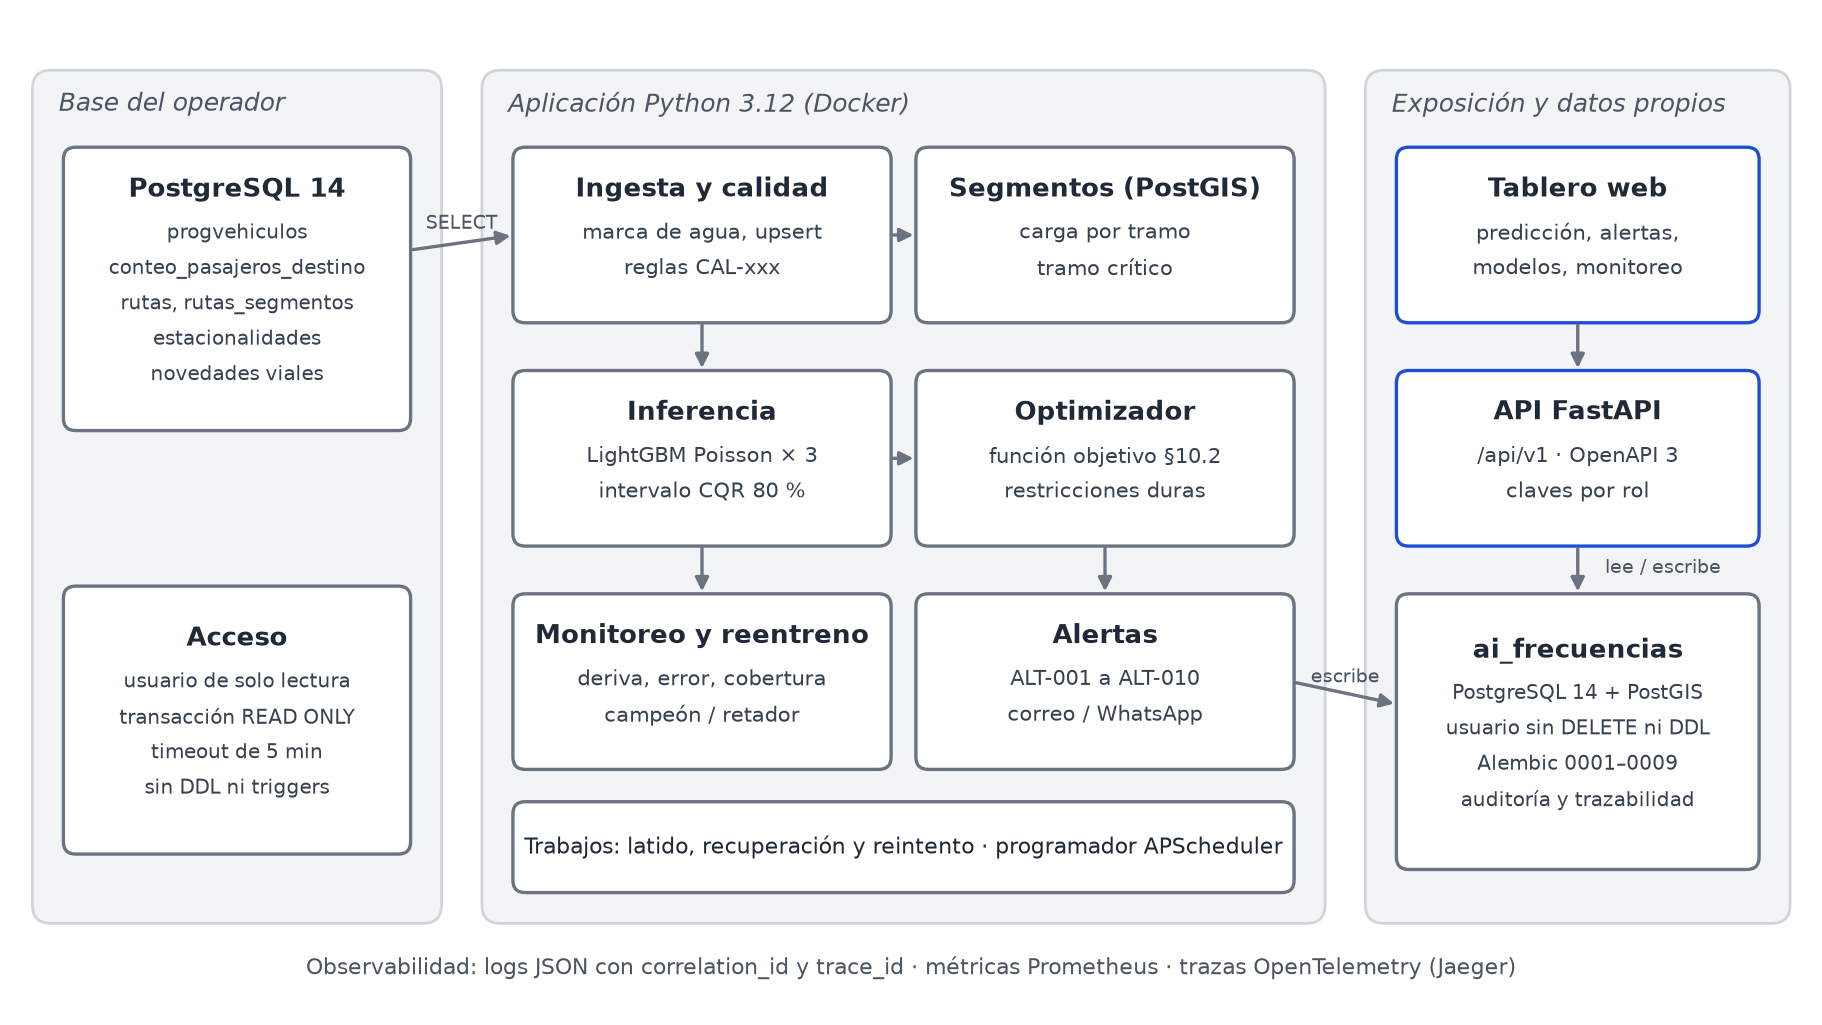
\includegraphics[width=\textwidth]{fig/arquitectura.png}
\caption{Componentes y flujo de datos. La base del operador solo se lee; todos los resultados se escriben en \cod{ai\_frecuencias}.}
\end{figure}

\subsection{Principios}

\begin{itemize}
  \setlength{\itemsep}{0.1em}
  \item \textbf{Separación de responsabilidades.} Cada paquete Python atiende una capa (Tabla~\ref{tab:componentes}). La API y el programador usan los mismos servicios de dominio.
  \item \textbf{No interferencia.} La base del operador se lee con un usuario de solo lectura, transacciones \cod{READ ONLY} y \cod{statement\_timeout} de 5 minutos. Nunca se ejecuta DDL ni DML sobre ella.
  \item \textbf{Mínimo privilegio en la base propia.} La aplicación escribe con un usuario que no puede truncar ni alterar tablas, ni borrar historia; solo puede reemplazar el perfil derivado \cod{segment\_profile}. Solo las migraciones usan al dueño del esquema.
  \item \textbf{Procesos largos como trabajos.} La ingesta, la predicción por lotes y el reentrenamiento corren fuera de las peticiones HTTP, con estado, avance, latido, recuperación y reintento.
  \item \textbf{Configuración externa.} Todo parámetro de entorno va en variables. Todo umbral de negocio va versionado en PostgreSQL. No hay secretos en el repositorio.
  \item \textbf{Trazabilidad.} Cada predicción, recomendación y alerta apunta a la ejecución, el modelo, las variables y la regla que la produjeron.
\end{itemize}

\begin{table}[H]
\centering\small
\caption{Componentes lógicos y tecnología.}\label{tab:componentes}
\begin{tabularx}{\textwidth}{lYl}
\toprule
\textbf{Componente} & \textbf{Responsabilidad} & \textbf{Tecnología} \\
\midrule
API REST & Autenticación por rol, validación, consultas, comandos, OpenAPI 3 & FastAPI, Pydantic \\
Acceso a la fuente & Consultas incrementales parametrizadas, solo lectura & SQLAlchemy 2.1, psycopg2 \\
Calidad y variables & Reglas CAL-xxx, serie de 15 min, 22 variables sin fuga & pandas, NumPy \\
Inferencia & Carga verificada por SHA-256, cuantiles CQR, explicación local & LightGBM 4.7 \\
Optimización & Función objetivo con restricciones duras (§10.2) & Python (búsqueda entera exacta) \\
Alertas & Reglas, deduplicación, estados, notificación & Motor propio, SMTP, WhatsApp Cloud API \\
Programación & Ciclo por cron, reintentos, reanudación & APScheduler \\
Persistencia & Esquema \cod{ai\_frecuencias}, migraciones, rol de aplicación & PostgreSQL 14, PostGIS 3.5, Alembic \\
Observabilidad & Logs JSON, métricas, trazas & structlog, Prometheus, OpenTelemetry \\
Calidad del código & Pruebas, cobertura, análisis estático & pytest, unittest.mock, SonarQube \\
\bottomrule
\end{tabularx}
\end{table}

\subsection{Despliegue}

Docker Compose define:

\begin{itemize}
  \item \cod{db}: PostgreSQL 14 con PostGIS.
  \item \cod{migraciones}: una sola corrida con el dueño del esquema; aplica Alembic y crea el usuario restringido.
  \item \cod{api}: arranca solo si las migraciones terminaron bien, con el usuario restringido.
  \item Perfiles opcionales: \cod{programador}, \cod{observabilidad} (Jaeger) y \cod{calidad} (SonarQube).
\end{itemize}

La imagen corre como usuario sin privilegios. Los modelos se montan desde \cod{modelos/}. La integración continua (GitHub Actions) tiene tres trabajos:

\begin{itemize}
  \item \textbf{Pruebas:} aplica, revierte y reaplica las migraciones y corre las pruebas.
  \item \textbf{Calidad:} levanta su propio servidor SonarQube y falla con hallazgos críticos o bloqueantes.
  \item \textbf{Imagen:} construye la imagen Docker.
\end{itemize}

\section{Datos}

\subsection{Fuentes y decisión sobre los consolidados}

La demanda se construye a partir de \cod{conteo\_pasajeros\_destino}: 176 millones de lecturas de sensores entre 2023 y 2025. Se une con \cod{progvehiculos} por \cod{idprogramacion} y se agrega por ruta y franja de 15 minutos. Los consolidados \cod{timbradas\_*} que propone la especificación no se usaron como fuente del modelo, por dos razones:

\begin{itemize}
  \item \cod{timbradas\_segmentos} solo cubre ocho semanas de 2023.
  \item Sus horas están desplazadas dos horas respecto de los sensores: la correlación franja a franja sube de 0,47 a 0,71 al corregir el desfase.
\end{itemize}

La suma de lecturas por viaje tiene correlación 0,9999 con \cod{numeropasajeros} de la programación.

Los scripts de segmentación del operador escriben en la base, así que no se pueden ejecutar con acceso de solo lectura. Su lógica se replicó con PostGIS: asignación de cada lectura al segmento más cercano con índice GiST y carga balanceada. Coincide en 99,7\,\% con \cod{timbradas\_segmentos}.

\subsection{Calidad}

Las reglas de calidad se derivan del análisis exploratorio. Cubren:

\begin{itemize}
  \item días sin lecturas, que se tratan como faltantes y no como cero;
  \item lecturas imposibles y saltos del contador acumulado;
  \item sensor de bajadas poco fiable;
  \item viajes con fin anterior al inicio;
  \item relaciones faltantes;
  \item distancias de lectura a la ruta mayores a 300 m.
\end{itemize}

Cada problema queda en \cod{data\_quality\_issue} con regla, dimensión (completitud, validez, consistencia, oportunidad, relacional), fila y causa. Se consulta por lote en \cod{GET /api/v1/data-quality}.

\subsection{Lectura incremental}

El ciclo lee desde la última franja del histórico: \cod{max(demand\_history.ts)} + 15 min. La carga es un upsert por clave natural, así que repetir un lote no duplica: se probó con 808.345 registros. Cada lote queda en \cod{execution\_log} con su ventana. Si un ciclo cae después de ingerir, el siguiente procesa desde la marca de agua del último ciclo exitoso, con un tope de 7 días; así no se pierden predicciones ni alertas. El mapa completo de tablas, consultas y planes de ejecución está en E07.

\subsection{Esquema propio}

El esquema \cod{ai\_frecuencias} tiene 17 tablas, todas creadas con Alembic, en \cod{TIMESTAMPTZ} y con claves naturales protegidas por \cod{UNIQUE}:

\begin{itemize}
  \item histórico analítico (\cod{demand\_history}, \cod{trip\_history});
  \item resultados (\cod{prediction}, \cod{feature\_snapshot}, \cod{recommendation}, \cod{alert}, \cod{alert\_history}, \cod{notification});
  \item gobierno (\cod{model\_registry}, \cod{operational\_parameter}, \cod{api\_key});
  \item operación (\cod{execution\_log}, \cod{data\_quality\_issue}, \cod{monitoring\_metric});
  \item segmentación (\cod{route\_segment} con geometría PostGIS, \cod{segment\_observation}, \cod{segment\_profile}).
\end{itemize}

\section{Modelo de demanda}

\subsection{Formulación y entrenamiento}

Pronóstico supervisado de subidas por ruta y franja, con un modelo LightGBM de objetivo Poisson por horizonte (30, 60 y 120 min):

\begin{itemize}
  \item \textbf{Variables.} 22 variables que solo usan información anterior al instante de predecir: rezagos del mismo día, día anterior, semana y año; promedio de 4 semanas; minuto del día; tipo de día y festivos; estacionalidades; viajes habituales e impacto de novedades. Una prueba automática altera el futuro y verifica que la predicción no cambie.
  \item \textbf{División cronológica.} Entrenamiento, validación y prueba reservada, de mayo a noviembre de 2025.
  \item \textbf{Ajuste.} Hiperparámetros con Optuna (15 intentos, validación temporal de 4 pliegues, semilla 42).
  \item \textbf{Registro.} Datos, semilla, hiperparámetros, versión de variables, métricas, artefacto y su SHA-256 quedan en \cod{model\_registry}.
\end{itemize}

\begin{table}[H]
\centering\small
\caption{Error en el periodo de prueba (mayo a noviembre de 2025, 44.626 franjas).}
\begin{tabular}{lrrrr}
\toprule
\textbf{Horizonte} & \textbf{WAPE modelo} & \textbf{WAPE base 4 sem.} & \textbf{WAPE sem. pasada} & \textbf{MAE modelo / base} \\
\midrule
30 min & 10,1\,\% & 14,9\,\% & 18,4\,\% & 16,9 / 24,9 \\
60 min & 10,5\,\% & 14,9\,\% & 18,4\,\% & 17,6 / 24,9 \\
120 min & 10,8\,\% & 14,9\,\% & 18,4\,\% & 18,2 / 24,9 \\
\bottomrule
\end{tabular}
\end{table}

El reporte por ruta, tipo de día y hora (pico y valle) y el sesgo están en \cod{modelos/reporte\_entrenamiento.json} y en el artículo técnico (\cod{paper/main.pdf}). En días especiales el error es de 14--16\,\%, frente a 99\,\% de la línea base.

\subsection{Incertidumbre y explicabilidad}

Los cuantiles p10 y p90 se calibran con predicción conforme (CQR). El intervalo del 80\,\% cubre 81,6--82,5\,\% en prueba. Fuera del servicio habitual el intervalo se marca como no calibrado.

Cada predicción guarda las variables usadas (\cod{feature\_snapshot}) y una explicación local: el efecto porcentual de las variables más influyentes, por ejemplo ``hora del día +38\,\%''. La importancia global (ganancia y SHAP) está en el reporte de entrenamiento.

\subsection{Ciclo de vida, monitoreo y aprendizaje continuo}

\textbf{Carga verificada.} El modelo se carga una vez y se verifica su huella; un paquete alterado se rechaza.

\textbf{Monitoreo (§9.4).} En cada ciclo se calculan y guardan en \cod{monitoring\_metric}:

\begin{itemize}
  \item deriva de datos: PSI de las subidas recientes frente a las 8 semanas previas al corte del modelo;
  \item error móvil (WAPE de 7 días);
  \item cobertura del intervalo;
  \item volumen de predicciones;
  \item porcentaje de alertas descartadas.
\end{itemize}

Último ciclo: WAPE de 11--13\,\%, cobertura de 76--81\,\% y PSI de 0,08--0,21.

\textbf{Reentrenamiento} (§9.5, RF-018, RF-019):

\begin{itemize}
  \item Se dispara por degradación (ALT-010 por error o cobertura), por deriva (PSI $>$ 0,25) o por periodicidad (7 días), con al menos 24 horas entre intentos.
  \item El candidato se entrena con los datos anteriores a una ventana de comparación que ninguno de los dos modelos vio.
  \item Solo se activa si mejora el WAPE o la desviación de Poisson sin empeorar la otra y supera a la línea base.
  \item El modelo anterior queda registrado para revertir con \cod{POST /models/\{id\}/activate}.
  \item Los paquetes reemplazados se archivan, no se borran.
\end{itemize}

\section{Optimización de frecuencia}

Para cada ruta y hora se eligen los buses por hora $b$ que minimizan la función objetivo de referencia (§10.2):
\begin{align*}
\min_{b \in \mathbb{Z}}\; & \alpha\, \frac{b\,T_c}{60} \;+\; \beta\, \frac{D}{2b} \;+\; \gamma\, \mathbb{E}\big[(L - b\,C\,o^{*})^{+}\big] \;+\; \delta\, |b - b_0| \\
\text{s.a.}\; & b \ge \lceil 60/H_{\max} \rceil, \qquad b\,C\,o_{c} \ge \mathbb{E}[L], \qquad b \le \lfloor 60/H_{\min} \rfloor, \qquad V(b) \le F,
\end{align*}

donde:

\begin{itemize}
  \item $T_c$ es la duración del ciclo de la ruta para el tipo de día y la franja;
  \item $D$ es la demanda prevista de la hora;
  \item $L = D \cdot f$ es la carga en el tramo más cargado ($f$ es el factor de carga medido por franja);
  \item $C$ es la capacidad;
  \item $o^{*}$ y $o_c$ son la ocupación objetivo (80\,\%) y la crítica (90\,\%);
  \item $b_0$ es la oferta actual, observada o habitual;
  \item $V(b)$ son los vehículos requeridos;
  \item $F$ es la flota disponible.
\end{itemize}

Los cuatro términos están en unidades equivalentes a una hora de operación de un vehículo:

\begin{itemize}
  \item costo de operación;
  \item horas de espera de los pasajeros, con espera media igual a la mitad del headway;
  \item pasajeros esperados por encima de la ocupación objetivo;
  \item cambio frente a lo que se opera.
\end{itemize}

\textbf{Incertidumbre.} $L$ se modela como normal con media $\mathbb{E}[L]$ y desviación $(p_{90} - p_{50})\,f / 1{,}2816$, tomadas del intervalo del modelo. El exceso esperado tiene forma cerrada $\sigma\varphi(z) + (\mu - c)(1 - \Phi(z))$.

\textbf{Solución.} El dominio factible tiene a lo sumo 30 enteros, así que la búsqueda exhaustiva da el óptimo global de forma exacta y auditable. Para cada recomendación se guardan los componentes del costo, las tres mejores alternativas, la restricción que limita la decisión y la sensibilidad a cada peso multiplicado por 0,5 y por 2. Si las restricciones no se pueden cumplir, la recomendación se marca \emph{no viable} con su motivo, en lugar de forzar una cifra.

\textbf{Fin del servicio.} Para cada ruta y día se calcula la ventana de despachos:

\begin{itemize}
  \item \textbf{Apertura:} la menor entre la primera salida programada del día y la mediana de las 4 semanas previas del mismo día de la semana.
  \item \textbf{Cierre:} la mayor entre la última salida programada del día y esa misma mediana.
\end{itemize}

Las horas con menos de 25\,\% dentro de la ventana no se recomiendan, y en la hora parcial los buses operados se comparan como tasa dentro del servicio. Así, después de la última salida el sistema no pide buses por el mínimo de servicio.

\textbf{Pesos y línea base.} Los pesos de referencia son $\alpha = 1$, $\beta = 0{,}1$, $\gamma = 1$ y $\delta = 0{,}5$. Están versionados en \cod{operational\_parameter} y requieren validación de SOBUSA. Con estos valores, recalculando las 666 horas-ruta del 1 al 14 de diciembre de 2025 con los modelos vigentes antes de esas fechas (\cod{pruebas/redistribucion.py}):

\begin{itemize}
  \item El óptimo coincide con la línea base de §10.3 ($\lceil$carga p90 / capacidad efectiva$\rceil$ con mínimo de servicio) en el 66\,\% de los casos y recomienda menos buses en el 34\,\%.
  \item Frente a lo operado, propone 8,7 buses por hora en promedio frente a 9,1.
  \item La flota se redistribuye: SILENCIO pasa de 8,4 a 6,8 buses por hora y CL 72 de 4,9 a 5,6.
  \item La mediana de ocupación esperada es 67\,\%.
\end{itemize}

\section{Alertas}

\begin{table}[H]
\centering\small
\caption{Catálogo implementado. Todos los umbrales se versionan en \cod{operational\_parameter}.}
\begin{tabularx}{\textwidth}{llY}
\toprule
\textbf{Código} & \textbf{Severidad} & \textbf{Condición} \\
\midrule
ALT-001 & preventiva / crítica & Carga p90 con la oferta actual $\ge$ umbral de capacidad; crítica si la recomendación no es viable \\
ALT-002 & crítica & Ocupación esperada con la oferta actual $\ge$ 90\,\% \\
ALT-003 & preventiva & Oferta actual menor que la recomendada, más allá de la tolerancia (2 buses/h y 15\,\%) \\
ALT-004 & informativa & Ocupación esperada $<$ 30\,\% con más buses de los recomendados \\
ALT-005 / 007 & preventiva & Demanda real fuera del intervalo con desvío $\ge$ 15\,\% \\
ALT-006 & crítica & En una hora, al menos 2 despachos programados y al menos 25\,\% salieron cancelados, sin iniciar o fuera de plazo (\cod{excedeplazosalida}) \\
ALT-008 & preventiva & Consolidado con valores atípicos \\
ALT-009 & crítica & Día sin lecturas, datos atrasados más de 2 periodos o fuente no disponible \\
ALT-010 & crítica & WAPE móvil $>$ tolerancia o cobertura del intervalo $<$ 65\,\%, con al menos 3 días observados \\
\bottomrule
\end{tabularx}
\end{table}

Cada alerta guarda empresa, ruta, ventana, horizonte, valor observado, esperado y umbral, puntuación de anomalía, explicación, variables influyentes, recomendación y referencias a la predicción, la recomendación, el modelo y la ejecución.

\begin{itemize}
  \item \textbf{Deduplicación.} Se hace por clave mientras la alerta está abierta.
  \item \textbf{Estados.} Abierta, reconocida, asignada, cerrada y descartada, con bitácora.
  \item \textbf{Notificación.} Las nuevas críticas se notifican por correo y WhatsApp, con timeout, reintento y circuit breaker.
\end{itemize}

ALT-006 da unas 4 alertas diarias entre las tres rutas con los datos de diciembre de 2025.

Para no saturar al operador, el tablero agrupa las alertas por ruta, código y día (en la demostración, 775 pendientes caben en 178 grupos) y permite gestionarlas en lote.

\section{API REST}

\textbf{Convenciones.}

\begin{itemize}
  \item Ruta base \cod{/api/v1}, JSON UTF-8 y fechas ISO-8601 con zona \cod{America/Bogota}.
  \item Validación con Pydantic.
  \item Errores uniformes: \cod{\{error:\{codigo, mensaje, detalle, correlation\_id\}\}}.
  \item Paginación (\cod{page}, \cod{size}) y filtros en las colecciones.
  \item Cabecera \cod{X-Correlation-Id} y autenticación por \cod{X-API-Key} con roles lector, operador y administrador.
  \item Swagger UI restringido por ambiente.
\end{itemize}

El contrato completo está en \cod{docs/openapi.json} (OpenAPI 3.1, 28 rutas).

\begin{longtable}{@{}p{0.44\textwidth}p{0.12\textwidth}p{0.38\textwidth}@{}}
\caption{Endpoints.}\\
\toprule
\textbf{Método y ruta} & \textbf{Rol} & \textbf{Finalidad} \\
\midrule
\endfirsthead
\toprule
\textbf{Método y ruta} & \textbf{Rol} & \textbf{Finalidad} \\
\midrule
\endhead
\cod{POST /frequency/executions} & operador & Lanzar el ciclo (202, trabajo asíncrono) \\
\cod{GET /frequency/executions[/\{id\}]} & lector & Estado, etapa, avance, intento, ventana, métricas, errores \\
\cod{POST /frequency/executions/\{id\}/retry} & operador & Reintentar un ciclo fallido o interrumpido \\
\cod{POST /predictions/run} & operador & Inferencia para ruta y referencia \\
\cod{GET /predictions[/\{id\}/segments]} & lector & Pronósticos por filtros; desagregación por segmento \\
\cod{POST /recommendations/calculate} & operador & Frecuencia y flota optimizadas \\
\cod{GET /recommendations} & lector & Recomendaciones por filtros \\
\cod{GET /overview} & lector & Resumen del día: acción por ruta para la hora actual y la siguiente, franja del día y alertas \\
\cod{GET /alerts[/summary|/\{id\}]} & lector & Alertas por estado, severidad, código, ruta, fecha y ventana \\
\cod{GET /alerts/groups} & lector & Alertas agrupadas por ruta, código, severidad y día \\
\cod{POST /alerts/status} & operador & Cambio de estado en lote (hasta 500), con bitácora por alerta \\
\cod{PATCH /alerts/\{id\}/status} & operador & Reconocer, asignar, comentar, cerrar o descartar \\
\cod{GET /models} · \cod{POST /models/\{id\}/activate} & lector · admin. & Registro de modelos; activación auditada \\
\cod{GET /monitoring[/history]} & lector & Métricas de monitoreo vigentes e histórico \\
\cod{GET /parameters} · \cod{PUT /parameters/\{clave\}} & lector · admin. & Umbrales y pesos versionados \\
\cod{GET /segments[/profile]} & lector & Catálogo y perfil de carga por segmento \\
\cod{GET /data-quality} · \cod{GET /notifications} & lector & Problemas de calidad por lote; envíos \\
\cod{GET /export/\{recurso\}} & lector & CSV o XLSX filtrado \\
\cod{GET /salud} · \cod{GET /metrics} & público & Salud y métricas Prometheus \\
\bottomrule
\end{longtable}

\section{Requisitos no funcionales}

\begin{longtable}{@{}p{0.17\textwidth}p{0.48\textwidth}p{0.29\textwidth}@{}}
\caption{Cumplimiento y evidencia.}\\
\toprule
\textbf{Requisito} & \textbf{Cómo se cumple} & \textbf{Evidencia} \\
\midrule
\endfirsthead
\toprule
\textbf{Requisito} & \textbf{Cómo se cumple} & \textbf{Evidencia} \\
\midrule
\endhead
RNF-001 Disponibilidad & Latido, recuperación de ejecuciones sin latido, reanudación automática y ventana pendiente desde la última marca exitosa & Ciclo real fallido y reintentado; API matada con \cod{docker kill} a mitad de un ciclo y reanudada sola (\cod{caida\_api.json}) \\
RNF-002 Rendimiento & Consultas paginadas indexadas; predicciones precalculadas por el ciclo & p95 de 146 ms con 10 usuarios (\cod{carga\_api.json}) \\
RNF-003 Ingesta & Upsert por lotes con \cod{COPY} a tabla temporal & 808.345 registros en 149 s, pico de 964 MB \\
RNF-004 Asincronía & Ciclo como trabajo con etapa, avance y reintento (API y programador); exclusión entre procesos por índice único & \cod{humo\_docker.json}: 202 y 409 \\
RNF-005 Escalabilidad & API sin estado de sesión; procesamiento por ruta y fecha & --- \\
RNF-006 Observabilidad & Logs JSON con \cod{correlation\_id} y \cod{trace\_id}, Prometheus, trazas OpenTelemetry de HTTP, SQL y etapas & \cod{tests/test\_trazas.py} \\
RNF-007 Mantenibilidad & Arquitectura modular, 410 pruebas, 80\,\% de cobertura & \cod{docs/evidencias/} \cod{reporte-pruebas.xml} \\
RNF-008 Portabilidad & Docker Compose con base, migraciones, API y perfiles & \cod{humo\_docker.json} \\
RNF-009 Compatibilidad & \cod{/api/v1}, OpenAPI 3.1, 11 migraciones reversibles probadas en CI & \cod{docs/openapi.json} \\
RNF-010 Resiliencia & Timeout, reintento con espera creciente y circuit breaker en fuente y notificaciones & \cod{tests/test\_resiliencia.py} \\
RNF-011 Trazabilidad IA & Ejecución, modelo, variables, regla y parámetros enlazados en cada salida & Esquema E07 \\
RNF-012 Accesibilidad & Navegación por teclado, contraste $\ge$ 5,7:1, modo oscuro y móvil & \cod{e2e\_tablero.json} \\
RNF-013 Calidad de código & SonarQube: 0 bugs, 0 vulnerabilidades, 0 code smells, 0 puntos de seguridad, 0,3\,\% de duplicación & \cod{sonarqube.json} \\
RNF-014 Pruebas en CI & GitHub Actions: pruebas con PostGIS y análisis con SonarQube propio & \cod{.github/workflows/ci.yml} \\
\bottomrule
\end{longtable}

\section{Decisiones técnicas}

\begin{longtable}{@{}p{0.22\textwidth}p{0.3\textwidth}p{0.42\textwidth}@{}}
\caption{Decisiones, alternativas consideradas y razones.}\\
\toprule
\textbf{Decisión} & \textbf{Alternativas} & \textbf{Razón} \\
\midrule
\endfirsthead
\toprule
\textbf{Decisión} & \textbf{Alternativas} & \textbf{Razón} \\
\midrule
\endhead
Sensores crudos como fuente de demanda & Consolidados \cod{timbradas\_*} & Los consolidados entregados cubren ocho semanas y tienen horas desplazadas; los sensores cubren tres años \\
LightGBM Poisson por horizonte & XGBoost, Random Forest, redes temporales & Cinco variantes de boosting difieren en décimas de punto; LightGBM es el más rápido. La mejora viene de los datos, no de la familia \\
Intervalos CQR & Cuantiles sin calibrar, ancho constante & Mejor cobertura (82\,\%) con ancho similar \\
Búsqueda exacta para la frecuencia & OR-Tools, SciPy MILP, PuLP & Dominio de a lo sumo 30 enteros por hora: óptimo global exacto, sin dependencias y auditable. Si se agrega flota compartida entre rutas, el mismo modelo pasa a MILP \\
ALT-006 por hora con despachos fallidos & Huecos entre salidas & \cod{fechasalida} es la hora programada; contar cancelados, sin iniciar y fuera de plazo (marca del operador) mide la falla real y da unas 4 alertas al día \\
Índice único parcial para un ciclo a la vez & Candado en memoria, \cod{pg\_advisory\_lock} & Funciona entre procesos y máquinas, sobrevive a reinicios y es visible en la tabla \\
Latido por instancia & Solo tiempo de inicio & Distingue un ciclo largo (reentrenamiento) de uno abandonado \\
Usuario de aplicación sin DDL y con DELETE solo en \cod{segment\_profile} & Usuario dueño & Mínimo privilegio; la historia no se puede borrar y el perfil es un resumen derivado que cada ciclo reemplaza \\
API que arranca sin modelos y lo informa & Detener el arranque & Un clon limpio no trae datos ni modelos: \cod{/salud} explica qué falta y nunca se presentan datos sintéticos como reales \\
Modelos y datos en un paquete privado & Publicarlos en el repositorio & Son datos del operador y artefactos con huella; el paquete reproduce la demostración sin acceso a su base \\
Sin columna de sentido & Inventar una regla de ida y vuelta & La guía no la define y las tres rutas son circuitos cerrados: el número de segmento ya ordena el recorrido \\
Demanda por segmento como reparto & Un modelo por segmento & Las observaciones por segmento cubren desde noviembre de 2025; alcanzan para repartir con cuotas, no para entrenar \\
Verificador SCRAM generado en cliente & \cod{ALTER ROLE ... PASSWORD} en claro & La clave no viaja ni queda en logs del servidor \\
Modelos fuera de git & Versionarlos en el repositorio & Son artefactos con huella registrada; git alteraba sus fines de línea \\
SonarQube como servicio del job de CI & Servidor externo con secretos & Reproducible y sin credenciales externas \\
Instrumentación SQLAlchemy con \cod{skip\_dep\_check} & Fijar SQLAlchemy 2.0 & La instrumentación declara soporte hasta 2.0; con 2.1 funciona y está cubierta por pruebas \\
\bottomrule
\end{longtable}

\section{Riesgos y pendientes}

\begin{itemize}
  \setlength{\itemsep}{0.1em}
  \item \textbf{Parámetros operativos sin validar.} Capacidad (50 pasajeros), headway máximo (10 min de día) y pesos de la función objetivo. En 7--20\,\% de los viajes la carga medida supera 50 pasajeros. Mitigación: son parámetros versionados en la base y se ajustan sin desarrollo.
  \item \textbf{Fuente.} Si el operador corrige lecturas pasadas, el ciclo no las relee. Mitigación: recarga idempotente por rango (\cod{-{}-desde}, \cod{-{}-hasta}, \cod{-{}-origen base}). Pendiente: que el operador indique qué periodos cambiaron.
  \item \textbf{Demanda por segmento.} Es un reparto orientativo: WAPE de 44\,\% por segmento y hora en diciembre de 2025, con sesgo de +0,7\,\% al descontar la cobertura de 92,8\,\% de las observaciones.
  \item \textbf{Recaudo.} Se estiman pasajeros esperados y en riesgo de no abordar. Falta la tarifa del operador (\cod{tarifa\_pasajero}) para expresarlos en pesos.
  \item \textbf{Notificaciones simuladas} hasta recibir credenciales de SMTP y WhatsApp.
  \item \textbf{Una instancia de API por host,} supuesto de la recuperación al arrancar. Para varias réplicas, la recuperación queda solo por latido.
  \item \textbf{Video de demostración (E11)} a cargo del equipo, con el guion de \cod{docs/guion\_demo.md}.
\end{itemize}

\end{document}
